\item \textbf{{[}YIJC/PRELIM/9597/2019/P1/Q3{]} }

An \texttt{ExpressionTree} data structure is required to store 20
nodes. A linked list is maintained of all the nodes. A node contains
a data value and two pointers: a left pointer and a right pointer.
Items in the list are initially linked using their \texttt{LeftChild}
pointers. 

Each node is implemented as an instance of the class \texttt{Node}. 

The class \texttt{Node} has the following properties: Class: Node
Attributes Identifier Data Type Description DataValue STRING The node
data LeftChild INTEGER The left node pointer RightChild INTEGER The
right node pointer 

The \texttt{ExpressionTree} class is implemented as follows: Class:
ExpressionTree Attributes Identifier Data Type Description Tree ARRAY{[}1:20{]}
OF Node The tree data, initialised as a linked list Fringe ARRAY:
INTEGER A list to store the index of nodes traversed Root INTEGER
Index for the root position of the Tree array NextFreeChild INTEGER
Index for the next unused node 

The index of the first available node is indicated by \texttt{NextFreeChild}.
The initial value of \texttt{Root} is 0 and the initial value of \texttt{NextFreeChild}
is 0. The \texttt{Fringe} is initialised as an empty list and it will
be used for node insertion to store the index for the nodes traversed. 

The diagram shows the \texttt{Tree} array with the linked list to
record the unused nodes.
\begin{center}
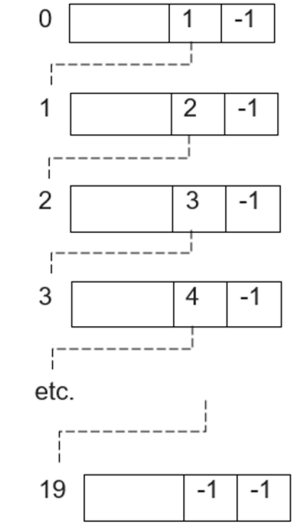
\includegraphics[width=0.15\paperwidth]{C:/Users/Admin/Desktop/Github/question_bank/LyX/static/img/9597-YIJC-2019-P1-Q3-1}
\par\end{center}

\subsection*{Task 3.1 }

Write a program code to define the \texttt{Node} and \texttt{ExpressionTree}
classes.

\subsection*{Evidence 3.1}

Your program code for Task 3.1. \hfill{}{[}12{]}

The task is to store the tokens of a binary arithmetic expression
in the data structure instantiated from the \texttt{ExpressionTree}
class. 

An arithmetic expression is a sequence of tokens that follows prescribed
rules. A token may be either an operand or an operator. 

A binary arithmetic operation using the standard arithmetic operators,
\texttt{+ - {*} /} , may be in the form of operand-operator-operand.
For example, 
\noindent \begin{center}
\texttt{2 + 3 }
\par\end{center}

where \texttt{2} and \texttt{3} are operands, \texttt{+} is an operator.
This expression will evaluate to a value of \texttt{5}. 

\subsection*{Task 3.2 }

Write a function \texttt{IsOperator(s)} that takes in a string \texttt{s},
and returns \texttt{True} if it is a standard arithmetic operator
and returns \texttt{False} if otherwise. 

\subsection*{Evidence 3.2 }

Your program code for Task 3.2. \hfill{}{[}2{]}

An expression tree is a binary tree with the following properties: 
\begin{enumerate}
\item[1.]  Each leaf is an \emph{operand}. 
\item[2.]  The root and internal nodes are \emph{operators}. 
\item[3.]  Subtrees are sub-expressions, with the root being an \emph{operator}.
\end{enumerate}
The following shows a series of commands to create and insert values
into the data structure to create an expression tree. 

\begin{minipage}[t]{0.5\columnwidth}%
\texttt{CreateNewExpTree }

\texttt{InsertToExpTree(\textquotedbl +\textquotedbl ) }

\texttt{InsertToExpTree(\textquotedbl{*}\textquotedbl ) }

\texttt{InsertToExpTree(\textquotedbl 4\textquotedbl ) }

\texttt{InsertToExpTree(\textquotedbl 2\textquotedbl ) }

\texttt{InsertToExpTree(\textquotedbl /\textquotedbl ) }

\texttt{InsertToExpTree(\textquotedbl 3\textquotedbl )}

\texttt{InsertToExpTree(\textquotedbl 1\textquotedbl )}%
\end{minipage}

The figure below shows the expression tree obtained and its \textbf{infix}
expression obtained by an in-order traversal. 

This expression will evaluate to \texttt{10}.
\begin{center}
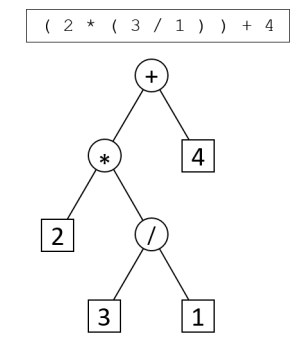
\includegraphics[width=0.25\paperwidth]{C:/Users/Admin/Desktop/Github/question_bank/LyX/static/img/9597-YIJC-2019-P1-Q3-2}
\par\end{center}

The following pseudocode (available in \texttt{PSEUDOCODE\_TASK\_3\_3.TXT})
can be used to add a node to the expression tree. 

\begin{minipage}[t]{0.88\columnwidth}%
\texttt{PROCEDURE Insert(NewToken)}

\texttt{\qquad{}IF NextFreeChild = -1 THEN // check if tree is full }

\texttt{\qquad{}\qquad{}RETURN 'Tree is Full'}

\texttt{\qquad{}// tree is not full, safe to insert new token }

\texttt{\qquad{}IF NextFreeChild = 0 THEN // inserting into empty
Tree }

\texttt{\qquad{}\qquad{}Tree{[}Root{]}.DataValue NewToken }

\texttt{\qquad{}\qquad{}NextFreeChild }

\texttt{\qquad{}\qquad{}Tree{[}Root{]}.LeftChild Tree{[}Root{]}.LeftChild
-1}

\texttt{\qquad{}ELSE }

\texttt{\qquad{}\qquad{}// inserting into tree with existing }

\texttt{\qquad{}\qquad{}// starting with Root }

\texttt{\qquad{}\qquad{}Current 0 // index of the current node }

\texttt{\qquad{}\qquad{}Previous -1 // index of previous node }

\texttt{\qquad{}\qquad{}NewNode Tree{[}NextFreeChild{]} // declare
new node }

\texttt{\qquad{}\qquad{}NewNode.DataValue NewToken }

\texttt{\qquad{}\qquad{}\qquad{}// Finding the node at which the
NewNode can be inserted }

\texttt{\qquad{}\qquad{}\qquad{}WHILE Current <> -1 THEN }

\texttt{\qquad{}\qquad{}\qquad{}\qquad{}CurrNode Tree{[}Current{]} }

\texttt{\qquad{}\qquad{}\qquad{}IF IsOperator(CurrNode.DataValue)
THEN }

\texttt{\qquad{}\qquad{}\qquad{}// check if CurrNode contains an
operator }

\texttt{\qquad{}\qquad{}\qquad{}\qquad{}IF CurrNode.LeftChild
= -1 THEN }

\texttt{\qquad{}\qquad{}\qquad{}\qquad{}// if LeftChild is empty,
insert here }

\texttt{\qquad{}\qquad{}\qquad{}\qquad{}\qquad{}CurrNode.LeftChild
NextFreeChild }

\texttt{\qquad{}\qquad{}\qquad{}\qquad{}\qquad{}NextFreeChild
NewNode.LeftChild }

\texttt{\qquad{}\qquad{}\qquad{}\qquad{}\qquad{}NewNode.LeftChild
-1 }

\texttt{\qquad{}\qquad{}\qquad{}\qquad{}\qquad{}Current -1}

\texttt{\qquad{}\qquad{}\qquad{}\qquad{}ELIF CurrNode.RightChild
= -1 THEN}

\texttt{\qquad{}\qquad{}\qquad{}\qquad{}\qquad{}// if RightChild
is empty, insert here }

\texttt{\qquad{}\qquad{}\qquad{}\qquad{}\qquad{}CurrNode.RightChild }

\texttt{\qquad{}\qquad{}\qquad{}\qquad{}\qquad{}NextFreeChild
NextFreeChild \textleftarrow{} NewNode.LeftChild }

\texttt{\qquad{}\qquad{}\qquad{}\qquad{}\qquad{}NewNode.LeftChild
-1}

\texttt{\qquad{}\qquad{}\qquad{}\qquad{}\qquad{}Current -1 }

\texttt{\qquad{}\qquad{}\qquad{}\qquad{}ELIF IsOperator(Tree{[}CurrNode.LeftChild{]}.DataValue)
THEN }

\texttt{\qquad{}\qquad{}\qquad{}\qquad{}\qquad{}// if LeftChild
is an operator, }

\texttt{\qquad{}\qquad{}\qquad{}\qquad{}\qquad{}// traverse leftchild
subtree }

\texttt{\qquad{}\qquad{}\qquad{}\qquad{}\qquad{}Previous Current }

\texttt{\qquad{}\qquad{}\qquad{}\qquad{}\qquad{}Current CurrNode.LeftChild}

\texttt{\qquad{}\qquad{}\qquad{}\qquad{}\qquad{}Fringe.APPEND(Previous)}

\texttt{\qquad{}\qquad{}\qquad{}\qquad{}ELIF IsOperator(Tree{[}CurrNode.RightChild{]}.DataValue)THEN }

\texttt{\qquad{}\qquad{}\qquad{}\qquad{}\qquad{}// if RightChild
is an operator, }

\texttt{\qquad{}\qquad{}\qquad{}\qquad{}\qquad{}// traverse rightchild
subtree }

\texttt{\qquad{}\qquad{}\qquad{}\qquad{}\qquad{}Previous Current}

\texttt{\qquad{}\qquad{}\qquad{}\qquad{}\qquad{}Current CurrNode.RightChild }

\texttt{\qquad{}\qquad{}\qquad{}\qquad{}\qquad{}Fringe.APPEND(Previous) }

\texttt{\qquad{}\qquad{}\qquad{}\qquad{}ELSE // traverse right
subtree }

\texttt{\qquad{}\qquad{}\qquad{}\qquad{}\qquad{}Previous Fringe.POP(-1) }

\texttt{\qquad{}\qquad{}\qquad{}\qquad{}\qquad{}Current Tree{[}Previous{]}.RightChild}

\texttt{\qquad{}\qquad{}\qquad{}\qquad{}ENDIF }

\texttt{\qquad{}\qquad{}\qquad{}ELSE // no place to insert}

\texttt{\qquad{}\qquad{}\qquad{}\qquad{}RETURN \textquotedbl Cannot
be inserted\textquotedbl{} }

\texttt{\qquad{}\qquad{}\qquad{}ENDIF }

\texttt{\qquad{}\qquad{}ENDWHILE}

\texttt{\qquad{}ENDIF}

\texttt{ENDPROCEDURE}%
\end{minipage}

\subsection*{Task 3.3 }

Write a code to implement the \texttt{Insert} method for the \texttt{ExpressionTree}
class from this pseudocode.

You may use the text file \texttt{PSEUDOCODE\_TASK\_3\_3.TXT} as a
basis for writing your code.

\subsection*{Evidence 3.3 }

Your program code for Task 3.3. \hfill{}{[}7{]}

\subsection*{Task 3.4: }

Write a code for the \texttt{Display} method for the \texttt{ExpressionTree}
class which displays the contents of \texttt{Tree} in index order. 

\subsection*{Evidence 3.4 }

Your program code for Task 3.4. \hfill{} {[}4{]}

\subsection*{Task 3.5 }

Write a sequence of program statements to: 
\begin{itemize}
\item create an expression tree
\item add the data items based on the sequence of commands given 
\item display the array contents 
\end{itemize}

\subsection*{Evidence 3.5 }

Your program code for Task 3.5. \hfill{}{[}3{]}

\subsection*{Evidence 3.6 }

Screenshot showing the output from running the program in Task 3.5.
\hfill{}{[}1{]}

\subsection*{Task 3.6 }

The infix notation can be obtained by performing an in-order traversal
in the expression tree. 

Write a code for the \texttt{infix} method for the \texttt{ExpressionTree}
class to generate the infix notation for a complete expression tree. 

\subsection*{Evidence 3.7 }

Your program code for Task 3.6. \hfill{} {[}6{]}

\subsection*{Evidence 3.8 }

Screenshot showing the output from running the program in Task 3.6.
\hfill{} {[}1{]}

\subsection*{Task 3.7 }

Write a code for the \texttt{calculate} method to evaluate and return
the numerical answer for the expression, rounded off to 2 decimal
places. 

\subsection*{Evidence 3.9 }

Your program code for Task 3.7. \hfill{}{[}3{]}

\subsection*{Evidence 3.10 }

Screenshot showing the output from running the program in Task 3.7.
\hfill{}{[}1{]}